\documentclass[border=18pt]{standalone}
\usepackage[T1]{fontenc}
\usepackage{tikz}
\usetikzlibrary{positioning,arrows.meta,fit,backgrounds,calc}

\definecolor{clsBlue}{HTML}{2C5AA0}
\definecolor{clsBg}{HTML}{E9F0F9}
\definecolor{ownGreen}{HTML}{1F7A5A}
\definecolor{ownBg}{HTML}{E4F3EC}
\definecolor{viewOr}{HTML}{C4600A}
\definecolor{viewBg}{HTML}{FCEBD7}
\definecolor{structPu}{HTML}{6B3FA0}
\definecolor{structBg}{HTML}{F1EAF9}
\definecolor{topoBand}{HTML}{D7D7D7}
\definecolor{physBand}{HTML}{CFE6CB}
\definecolor{hl}{HTML}{FFD35C}

\begin{document}
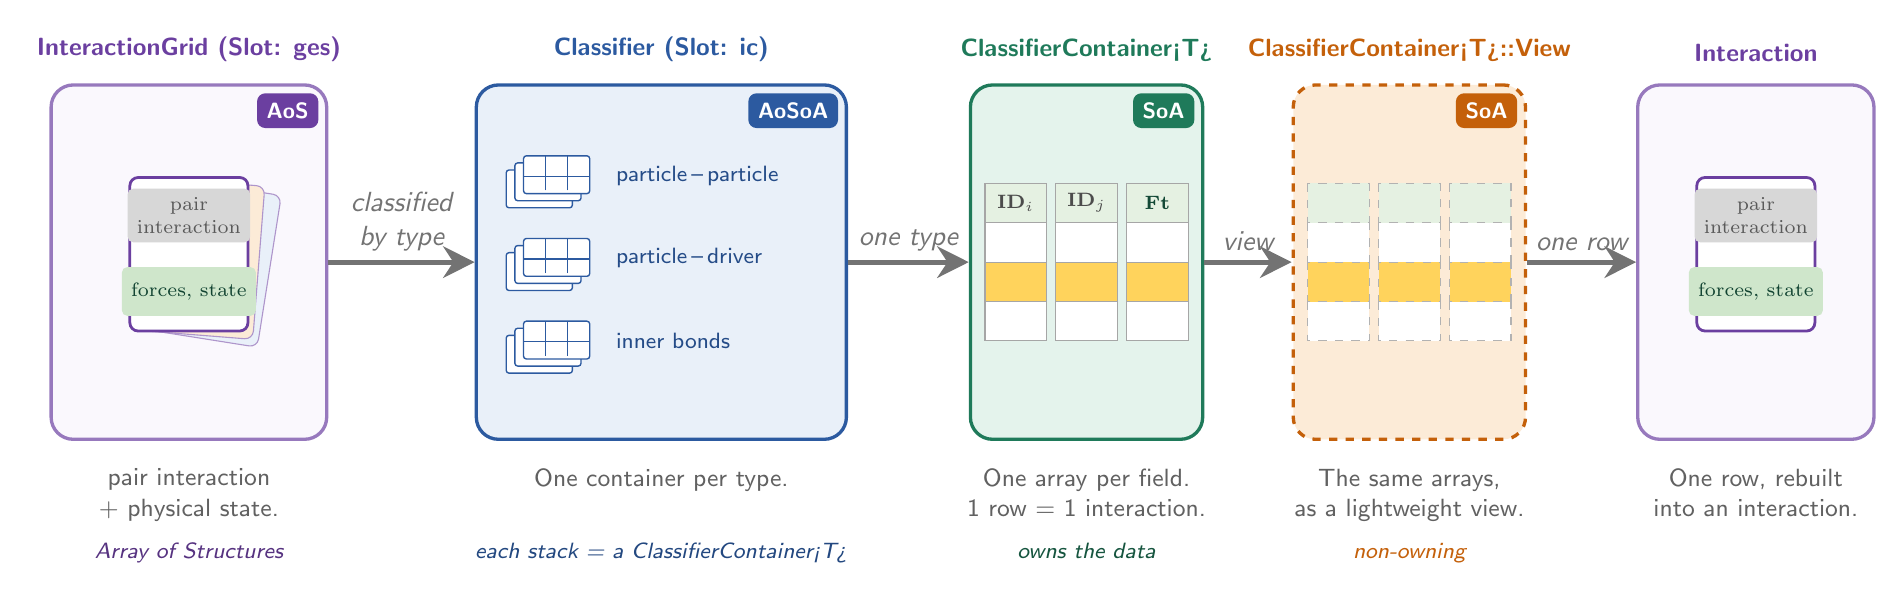
\begin{tikzpicture}[
  font=\sffamily,
  >=Stealth,
  stagetitle/.style={font=\sffamily\small\bfseries},
  capt/.style={font=\sffamily\small, text=black!62, align=center},
  subcapt/.style={font=\sffamily\footnotesize\itshape, align=center},
  bigbox/.style={rounded corners=8pt, line width=1.2pt},
  flow/.style={-{Stealth[length=4mm,width=4mm]}, line width=1.8pt, draw=black!55},
  flowlab/.style={font=\sffamily\itshape, text=black!55, align=center},
  pill/.style={rounded corners=3pt, text=white, font=\sffamily\footnotesize\bfseries, inner sep=3.5pt},
]

\def\titley{2.42}
\def\capty{-2.5}
\def\subcapty{-3.45}

% =============================================================
% STAGE 1 : INTERACTIONS
% =============================================================
\def\ax{0}
\begin{scope}[on background layer]
  \node[draw=structPu!70, bigbox, fill=structBg!35, minimum width=3.5cm, minimum height=4.5cm] (ibox) at (\ax,0){};
\end{scope}
\node[draw=structPu!55,fill=clsBg,rounded corners=3pt,minimum width=1.5cm,minimum height=1.95cm,rotate=-9]  at (\ax+0.28,0.0){};
\node[draw=structPu!55,fill=viewBg,rounded corners=3pt,minimum width=1.5cm,minimum height=1.95cm,rotate=-4.5] at (\ax+0.14,0.05){};
\node[draw=structPu,line width=1pt,fill=white,rounded corners=3pt,minimum width=1.5cm,minimum height=1.95cm] (fc) at (\ax,0.1){};
\node[fill=topoBand,rounded corners=2pt,minimum width=1.24cm,minimum height=0.66cm,font=\scriptsize,text=black!65,align=center] at ($(fc.north)+(0,-0.5)$){pair\\ interaction};
\node[fill=physBand,rounded corners=2pt,minimum width=1.24cm,minimum height=0.62cm,font=\scriptsize,text=ownGreen!55!black] at ($(fc.south)+(0,0.52)$){forces, state};
\node[pill, fill=structPu, anchor=north east] at ($(ibox.north east)+(-0.12,-0.12)$){AoS};
	\node[stagetitle, structPu, anchor=south] at (\ax,\titley){InteractionGrid (Slot: ges)};
\node[capt, anchor=north] at (\ax,\capty){pair interaction\\ + physical state.};
\node[subcapt, text=structPu!80!black, anchor=north] at (\ax,\subcapty){Array of Structures};

% =============================================================
% STAGE 2 : CLASSIFIER
% =============================================================
\def\sx{6.00}
\node[draw=clsBlue, bigbox, fill=clsBg, minimum width=4.7cm, minimum height=4.5cm] (cls) at (\sx,0){};
\node[pill, fill=clsBlue, anchor=north east] at ($(cls.north east)+(-0.12,-0.12)$){AoSoA};
	\node[stagetitle, clsBlue, anchor=south] at (\sx,\titley){Classifier (Slot: ic)};

\newcommand{\stk}[1]{%
  \foreach \o in {0,1,2}{
    \pgfmathsetmacro\dx{\o*0.11}\pgfmathsetmacro\dy{\o*0.09}
    \fill[white,draw=clsBlue,line width=0.5pt,rounded corners=1pt]
      ($(#1)+(-0.42+\dx,-0.26+\dy)$) rectangle ($(#1)+(0.42+\dx,0.22+\dy)$);}
  \draw[clsBlue,line width=0.4pt] ($(#1)+(-0.20,0.14)$)--($(#1)+(0.64,0.14)$);
  \draw[clsBlue,line width=0.4pt] ($(#1)+(0.08,-0.04)$)--($(#1)+(0.08,0.40)$);
  \draw[clsBlue,line width=0.4pt] ($(#1)+(0.36,-0.04)$)--($(#1)+(0.36,0.40)$);}

\coordinate (r1) at (\sx-1.55, 0.95);
\coordinate (r2) at (\sx-1.55,-0.10);
\coordinate (r3) at (\sx-1.55,-1.15);
\stk{r1}\stk{r2}\stk{r3}
\node[font=\sffamily\footnotesize, text=clsBlue!85!black, anchor=west] at ($(r1)+(0.85,0.15)$){particle\,--\,particle};
\node[font=\sffamily\footnotesize, text=clsBlue!85!black, anchor=west] at ($(r2)+(0.85,0.15)$){particle\,--\,driver};
\node[font=\sffamily\footnotesize, text=clsBlue!85!black, anchor=west] at ($(r3)+(0.85,0.15)$){inner bonds};

\node[capt, anchor=north] at (\sx,\capty){One container per type.};
\node[subcapt, text=clsBlue!80!black, anchor=north] at (\sx,\subcapty){each stack = a ClassifierContainer<T>};

% =============================================================
% table geometry : 3 SEPARATED columns  ->  reads as SoA (one array per field)
% =============================================================
\def\cw{0.78}\def\ch{0.5}\def\cg{0.12}\def\ncol{3}
\pgfmathsetmacro\tabw{\ncol*\cw+(\ncol-1)*\cg}

% =============================================================
% STAGE 3 : ClassifierContainer<T>  (owning SoA)
% =============================================================
\def\cx{11.4}
\pgfmathsetmacro\tx{\cx-\tabw/2}
\begin{scope}[on background layer]
  \node[draw=ownGreen, bigbox, fill=ownBg, minimum width=2.95cm, minimum height=4.5cm] (cont) at (\cx,0){};
\end{scope}
\foreach \c in {0,1,2}{
  \pgfmathsetmacro\xx{\tx+\c*(\cw+\cg)}
  % faint "array" cap on each column
  \foreach \r in {0,1,2,3}{
    \pgfmathsetmacro\yy{1.0-\r*\ch}
    \ifnum\r=2\def\cb{hl}\else\ifnum\r=0\def\cb{physBand!55!white}\else\def\cb{white}\fi\fi
    \fill[\cb,draw=black!35] (\xx,\yy) rectangle (\xx+\cw,\yy-\ch);}
}
\node[font=\scriptsize\bfseries, text=black!70] at ($(\tx,0.75)+(0.39,0)$){ID$_i$};
\node[font=\scriptsize\bfseries, text=black!70] at ($(\tx,0.75)+(1.29,0)$){ID$_j$};
\node[font=\scriptsize\bfseries, text=ownGreen!60!black] at ($(\tx,0.75)+(2.19,0)$){Ft};
\node[pill, fill=ownGreen, anchor=north east] at ($(cont.north east)+(-0.12,-0.12)$){SoA};
\node[stagetitle, ownGreen, anchor=south] at (\cx,\titley){ClassifierContainer<T>};
\node[capt, anchor=north] at (\cx,\capty){One array per field.\\ 1 row = 1 interaction.};
\node[subcapt, text=ownGreen!70!black, anchor=north] at (\cx,\subcapty){owns the data};

% =============================================================
% STAGE 4 : ClassifierContainer<T>::View  (non-owning, same SoA as spans)
% =============================================================
\def\vxc{15.5}
\pgfmathsetmacro\vx{\vxc-\tabw/2}
\begin{scope}[on background layer]
  \node[draw=viewOr, bigbox, dashed, fill=viewBg, minimum width=2.95cm, minimum height=4.5cm] (vw) at (\vxc,0){};
\end{scope}
\foreach \c in {0,1,2}{
  \pgfmathsetmacro\xx{\vx+\c*(\cw+\cg)}
  \foreach \r in {0,1,2,3}{
    \pgfmathsetmacro\yy{1.0-\r*\ch}
    \ifnum\r=2\def\cb{hl}\else\ifnum\r=0\def\cb{physBand!55!white}\else\def\cb{white}\fi\fi
    \fill[\cb,draw=black!30,dashed,line width=0.4pt] (\xx,\yy) rectangle (\xx+\cw,\yy-\ch);}
}
\node[pill, fill=viewOr, anchor=north east] at ($(vw.north east)+(-0.12,-0.12)$){SoA};
\node[stagetitle, viewOr, anchor=south] at (\vxc,\titley){ClassifierContainer<T>::View};
\node[capt, anchor=north] at (\vxc,\capty){The same arrays,\\ as a lightweight view.};
\node[subcapt, text=viewOr, anchor=north] at (\vxc,\subcapty){non-owning};

% =============================================================
% STAGE 5 : one INTERACTION, rebuilt from a row of the View
% =============================================================
\def\rx{19.9}
\begin{scope}[on background layer]
  \node[draw=structPu!70, bigbox, fill=structBg!35, minimum width=3.0cm, minimum height=4.5cm] (obox) at (\rx,0){};
\end{scope}
\node[draw=structPu,line width=1pt,fill=white,rounded corners=3pt,minimum width=1.5cm,minimum height=1.95cm] (oc) at (\rx,0.1){};
\node[fill=topoBand,rounded corners=2pt,minimum width=1.24cm,minimum height=0.66cm,font=\scriptsize,text=black!65,align=center] at ($(oc.north)+(0,-0.5)$){pair\\ interaction};
\node[fill=physBand,rounded corners=2pt,minimum width=1.24cm,minimum height=0.62cm,font=\scriptsize,text=ownGreen!55!black] at ($(oc.south)+(0,0.52)$){forces, state};
\node[stagetitle, structPu, anchor=south] at (\rx,\titley){Interaction};
\node[capt, anchor=north] at (\rx,\capty){One row, rebuilt\\ into an interaction.};

% =============================================================
% ARROWS
% =============================================================
\draw[flow] (ibox.east) -- node[flowlab, above]{classified\\ by type} (cls.west);
\draw[flow] (cls.east)  -- node[flowlab, above]{one type} (cont.west);
\draw[flow] (cont.east) -- node[flowlab, above]{view} (vw.west);
\draw[flow] (vw.east)   -- node[flowlab, above]{one row} (obox.west);

\end{tikzpicture}
\end{document}
